Let's talk about \textbf{branching decisions}. We have several types of branching decisions, described as follows:
\begin{enumerate}
    \renewcommand{\labelitemi}{-}
    \item \textbf{Unary branching}. \\ 
    Usually a branching decision consists of posting an \textbf{unary constraint} to a single decision variable.
    \item \textbf{Enumeration branching}. \\ 
    By enumeration branching we label a decision variable with a specific value. At the same time enumeration branching is divided into:
    \begin{itemize}
        \renewcommand{\labelitemi}{-}
        \item \textbf{d-way branching}. \\ 
        We create a separate branch for every possible assignment coming from the domain of the decision variable. More formally:
        $$ \text{one branch is generated by } X_ i = v_j \text{ } \forall v_j \in D(X_i) $$
        We do not instantiate all these branches at the same time. First of all, we start from the \textbf{left-most branch} ($X_i = v_1$) going down in the 
        search, only when we are backtracking we would create the second branch ($X_i = v_2$) and so on. \vspace{7pt}
        
        Note: the letter \textbf{d} in \textbf{d-way branching} stands for the cardinality of variable's domain. \vspace{3.5pt}
        \begin{center}
            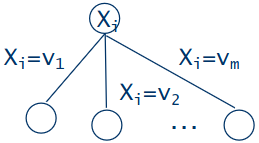
\includegraphics[width = 0.25\textwidth]{img/img13.png}
        \end{center} \vspace{3.5pt}
        \item \textbf{2-way branching}. \\
        In this case we define only two branches. The left-most branch is an assignment of whatever value coming from the domain and the failing counter-part
        is the no-assignment of this value to the decision variable. \vspace{3.5pt}
        \begin{center}
            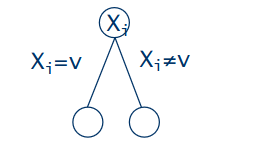
\includegraphics[width = 0.25\textwidth]{img/img14.png}
        \end{center} \vspace{3.5pt}
        If we encounter the failing part, the new node will be always the same decision variable but taking a different value from its domain.
    \end{itemize}
    The main difference between these approaches is that in \textbf{d-way branching} we have one node per variable, while in \textbf{2-way branching} we could have
    potentially a number of nodes equal to the cardinality of the domain ($|d|$).
\end{enumerate}
Exists also another way to do branching decisions without any assignment, based on restrictions of the domain:
\begin{enumerate}
    \setcounter{enumi}{2}
    \item \textbf{Domain partioning}. \\
    Simply, we define \textbf{partitions} of the domain of the decision variable and we state if the same decision variable can belong or not to one of these 
    partitions. Even in this case, domain partioning is divided into:
    \begin{itemize}
        \renewcommand{\labelitemi}{-}
        \item \textbf{k-way branching}. \\ 
        We create a specific number of partitions and we define among the branches if any given variable $X_i$ could belong or not to a partion $S_j$, where 
        $S_j \in D(X_i)$. \vspace{3.5pt}
        \begin{center}
            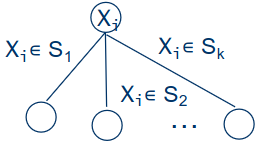
\includegraphics[width = 0.25\textwidth]{img/img15.png}
        \end{center} \vspace{3.5pt}
        \item \textbf{2-way branching}. \\ 
        It follows the same behavior as before: we start from the left-most branch assuming that the decision variable belongs to the partition $S$ ($X_i \in S$),
        if not we encounter the failing part and we determine a new 2-way branch with a different partition.
        \vspace{3.5pt}
        \begin{center}
            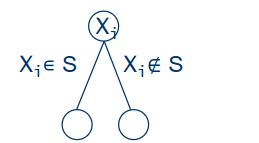
\includegraphics[width = 0.25\textwidth]{img/img16.png}
        \end{center} \vspace{3.5pt}
    \end{itemize}
\end{enumerate}
Most of times, solvers implement the \textbf{2-way branching} approach. By the way, the thing is: how do we know which decision variable $X_i$ should we pick? Or: 
which partition should we prefer? \vspace{7pt}

The answers to the previous questions are given by the \textbf{search heuristics}.